% \begin{figure*}[htb]
% \centering
% \subfigure[a] {\label{fig:ite}   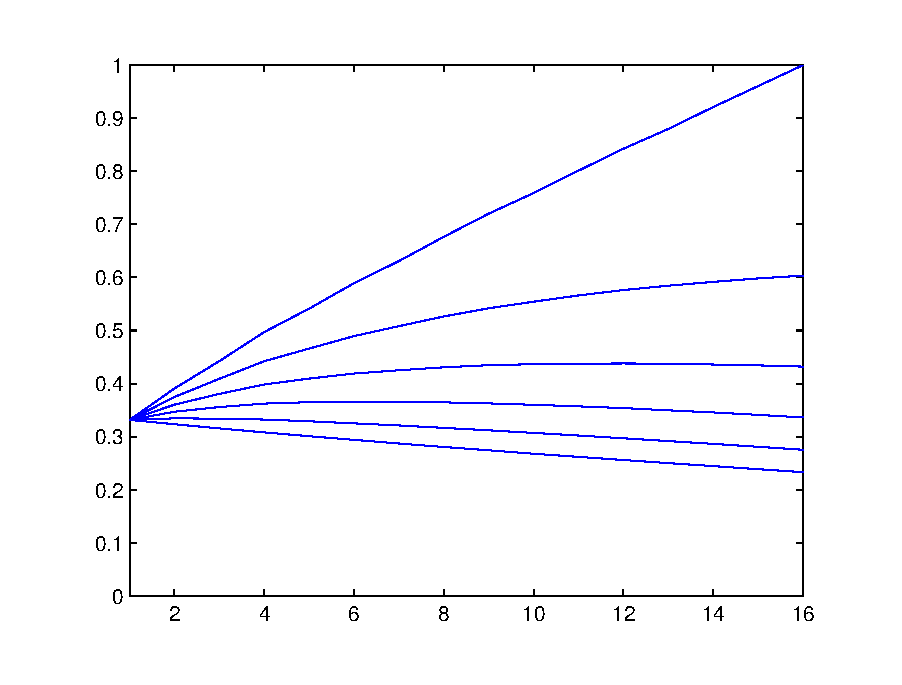
\includegraphics[width=0.32\textwidth]{fig/ppw_16_ite.eps}}%
% \subfigure[b] {\label{fig:taylor}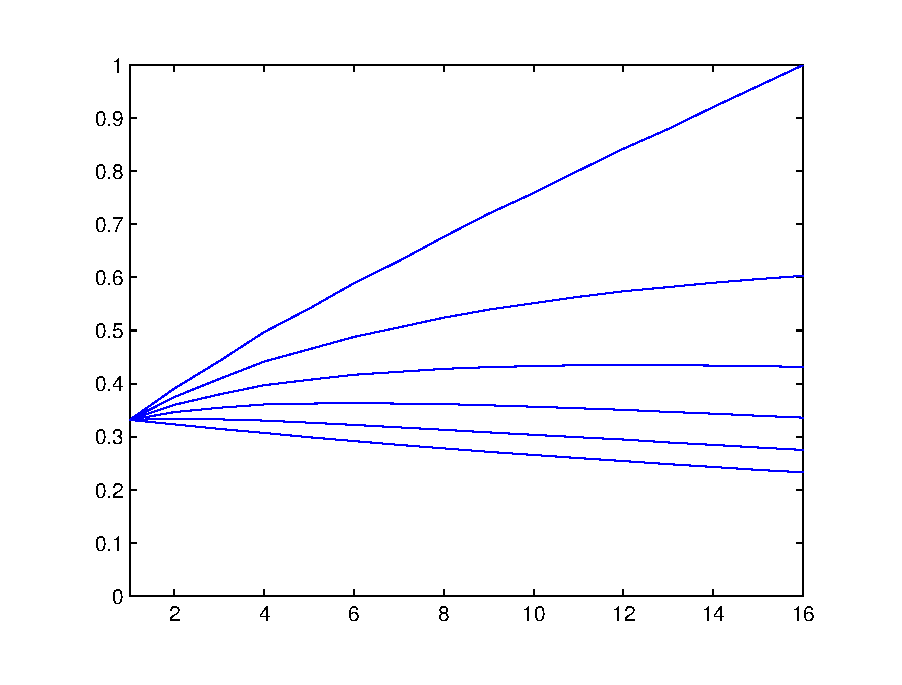
\includegraphics[width=0.32\textwidth]{fig/ppw_16_taylor.eps}}%
% \subfigure[c] {\label{fig:tayboo}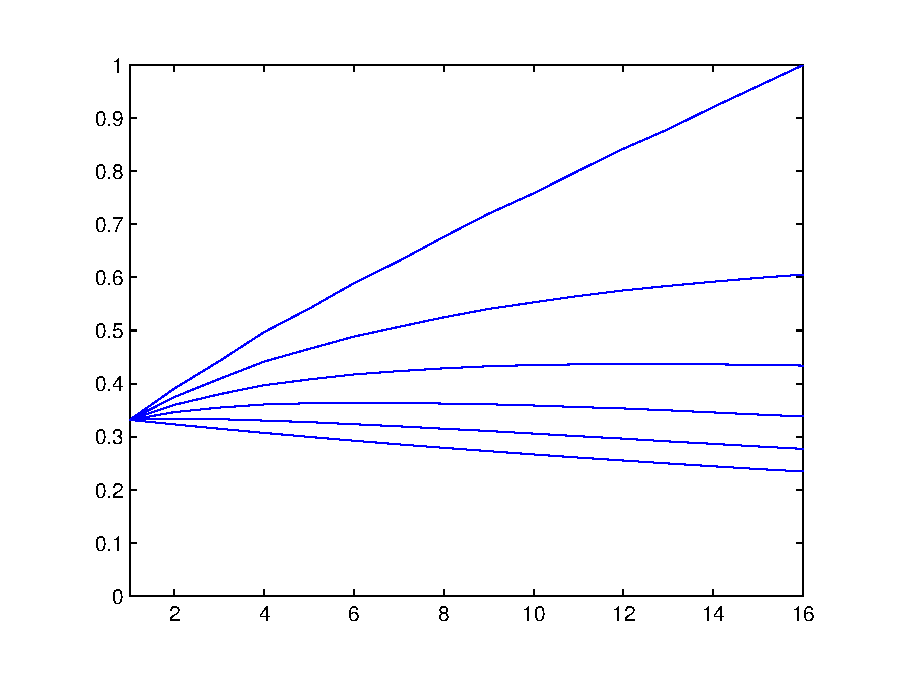
\includegraphics[width=0.32\textwidth]{fig/ppw_16_tayboo.eps}}
% \caption{PPW}  
% \label{fig:ppw}
% \end{figure*}

\begin{figure}
\centering
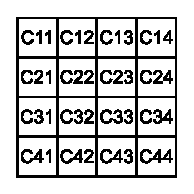
\includegraphics[width=0.5\linewidth]{fig/core_distribution.eps}
\caption{Configuration of the 16-core chip.}
\end{figure}

\section{Experimental Results}

In this section, we evaluate both accuracy and efficiency of the proposed light core distribution estimation method. 

\subsection{Experiment setup}
All data are collected on a PC with Intel I5 2400 CPU and 2 GB memory. In the experiment, multi-core systems with the number of cores ranging from 9 to 64 are used, and each system is tested with different parallel computation ratios. The thermal models of these systems are extracted from HotSpot [x] with default package and chip parameters. For all test cases, we set the ambient temperature as \SI{20}{\degreeCelsius}, and the thermal constraint as \SI{95}{\degreeCelsius}. Noted, for multi-core systems with different core numbers, the power density and power supply remain constant.

Through HSPICE simulation, the impact of temperature on device leakage can be characterized. With the collected data, we can obtain the parameters of model through curve fitting as shown in Fig.x.

For accuracy and speed comparison, we first perform the iteration based power estimation with brute force search strategy, which is accurate but very time-consuming, therefore we consider it as the golden accuracy baseline (called "golden" for short). Then, because our complete method includes two acceleration techniques (Taylor expansion based linear thermal models, and greedy based search strategy), we use two cases, in the first case, we implement the Taylor expansion based linear thermal models only, i.e., the non-iteration based power estimation method with brute force search strategy (called "lin-only" for short). In the second case, we further implement the greedy search strategy, i.e., the non-iteration based power estimation with greedy search strategy (called "lin \& greedy" for short). each with one more technique than the previous one, to better analyze our method. 

The schematic of the parallel operation is described here. The main core (the core in red) runs at all times, both in serial computation and parallel computation; while the other light cores only run during parallel segment of the code, they will be in idle state when executing the serial segment of the code. The remaining cores will always be off. The energy consumption is calculated according to this schematic.

\subsection{Estimation accuracy of the proposed method}

\begin{figure}%error trace

\centering


\subfloat[The estimated PPW curves by different methods for accuracy comparison when $f = 0.9$.]{
\label{fig:ppw_curves_comparison}
%\begin{minipage}[b]{0.4\textwidth}
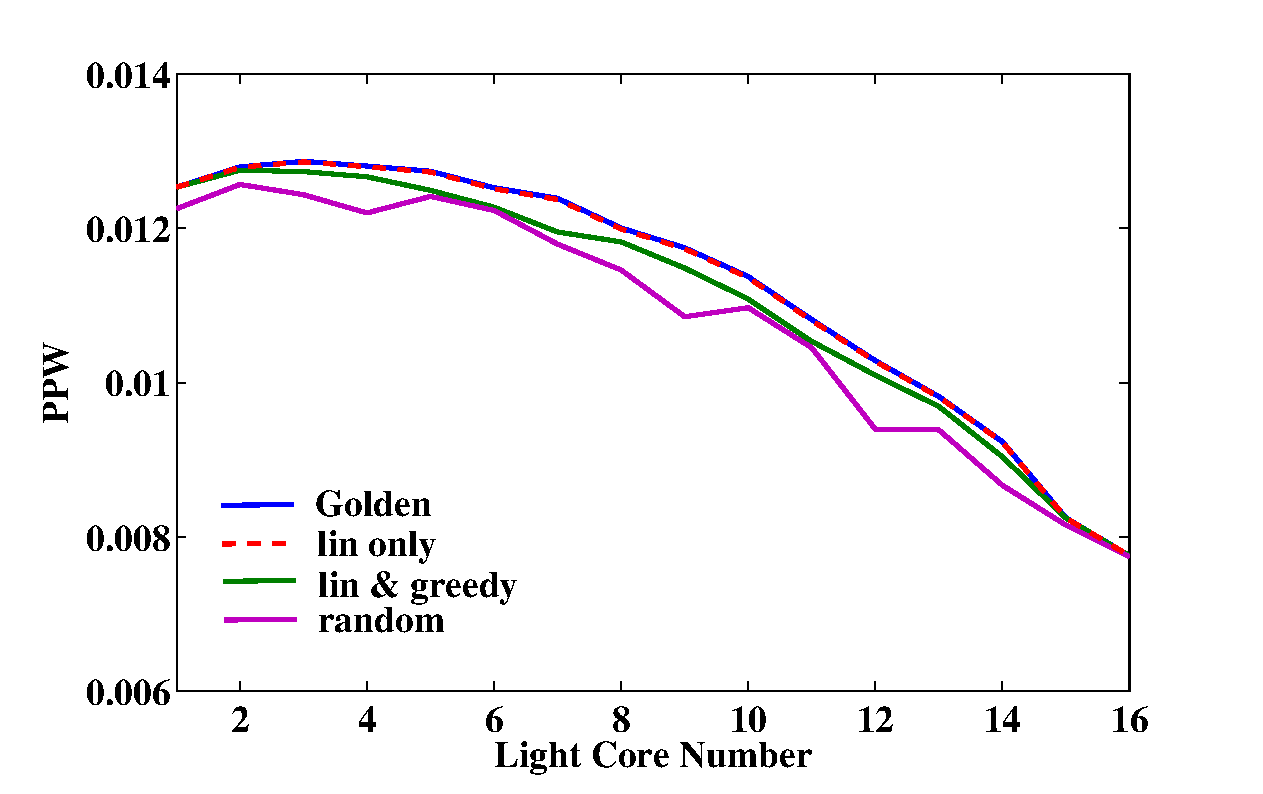
\includegraphics[width=1\columnwidth]{fig/ppw_accuracy_16.eps}
%\includegraphics[width=0.9\columnwidth]{fig_added/pd_trace3.eps}
%\end{minipage}
}

\subfloat[PPW estimation error curve of using ``lin only'' method.]{
\label{fig:ppw-err-linear}
%\begin{minipage}[b]{0.31\textwidth}
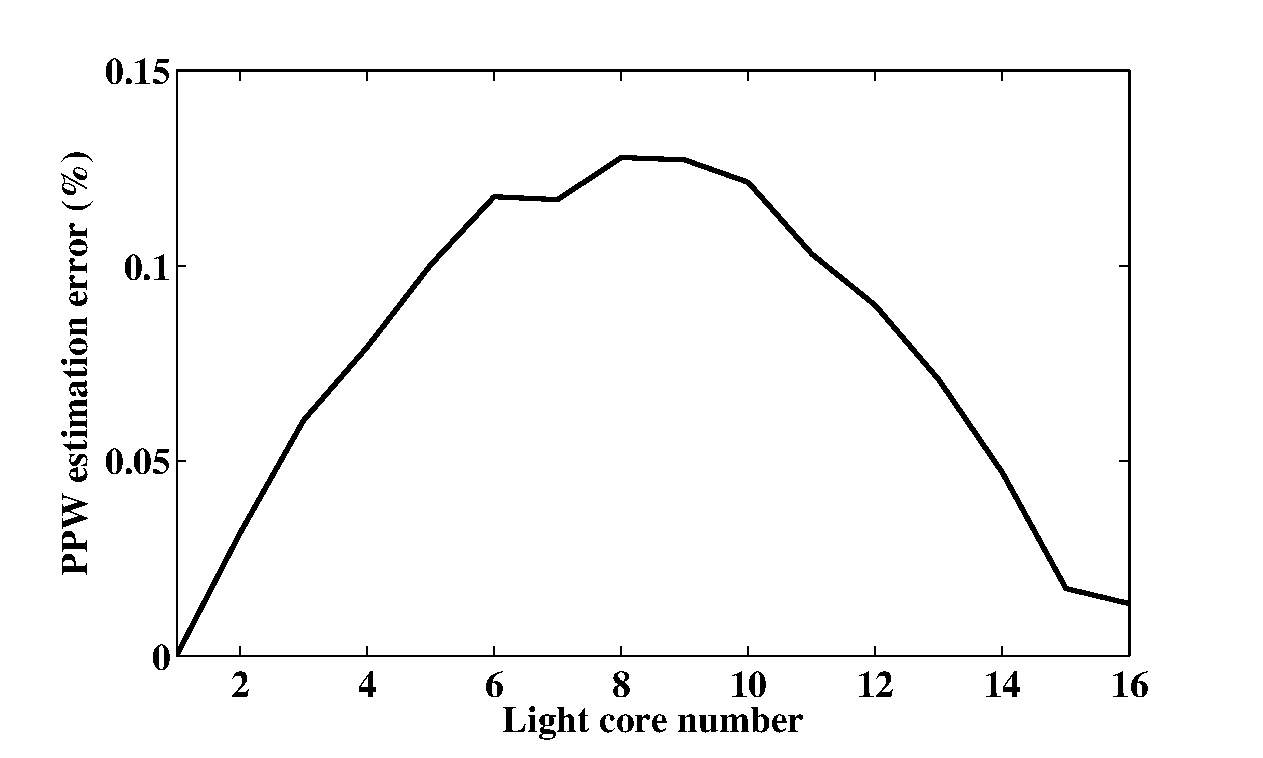
\includegraphics[width=1\columnwidth]{fig/ppw_err_tay_16.eps}
%\includegraphics[width=0.9\columnwidth]{fig_added/pd_trace3.eps}
%\end{minipage}
}

\subfloat[PPW estimation error curve of using ``lin \& greedy''
method.]{
\label{fig:ppw-err-boo}
%\begin{minipage}[b]{0.31\textwidth}
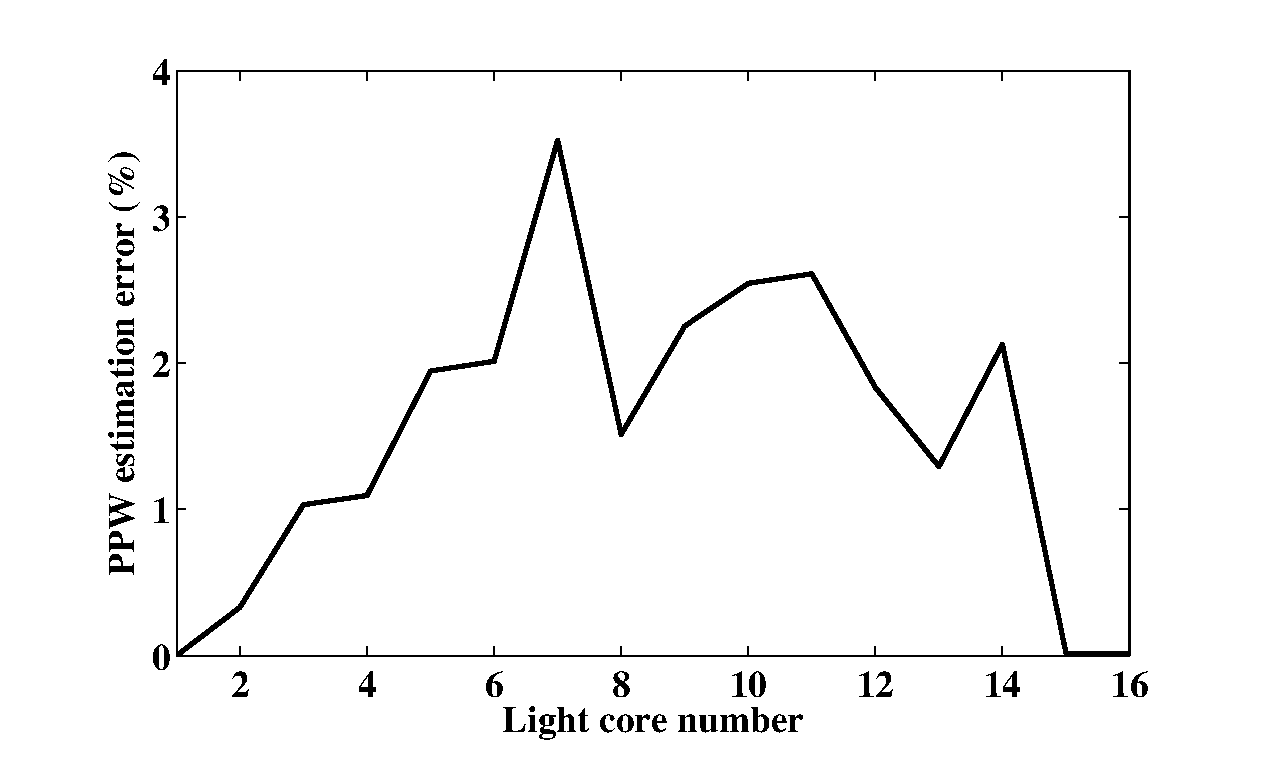
\includegraphics[width=1\columnwidth]{fig/ppw_err_boo_16.eps}
%\includegraphics[width=0.9\columnwidth]{fig_added/pd_trace3.eps}
%\end{minipage}
}

\subfloat[PPW estimation error curve of using ``random''
method.]{
\label{fig:ppw-err-random}
%\begin{minipage}[b]{0.31\textwidth}
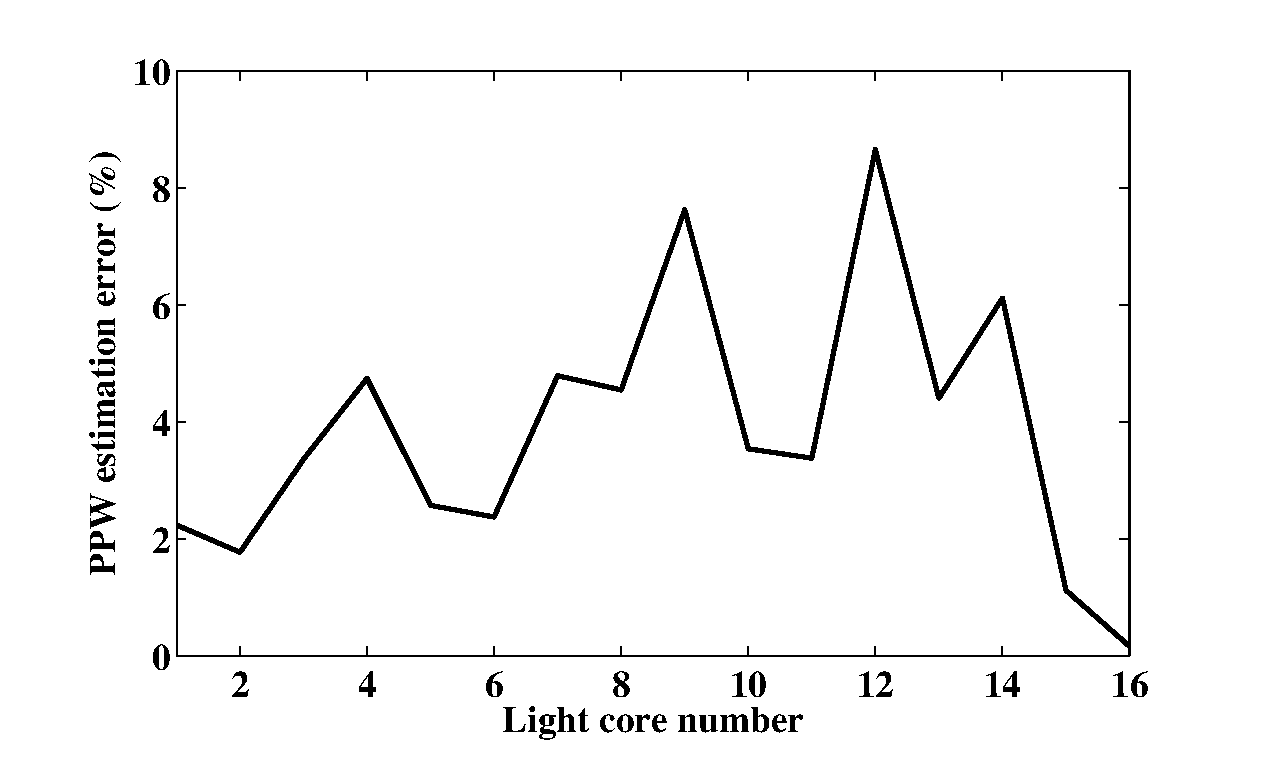
\includegraphics[width=1\columnwidth]{fig/ppw_err_random_16.eps}
%\includegraphics[width=0.9\columnwidth]{fig_added/pd_trace3.eps}
%\end{minipage}
}
\caption{Accuracy comparison and estimation error curves of
  the proposed method on the 16-core chip.}
\label{fig:error-curve}
\end{figure}



\begin{figure}%error trace

\centering

\subfloat[Golden light core distribution.]{
\label{fig:golden-map-16}
%\begin{minipage}[b]{0.31\textwidth}
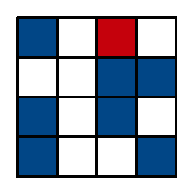
\includegraphics[width=0.35\columnwidth]{fig/map_ite_16_8.eps}
%\end{minipage}
}\qquad
\subfloat[Light core distribution of using ``lin-only''
method.]{
\label{fig:lin-map-16}
%\begin{minipage}[b]{0.31\textwidth}
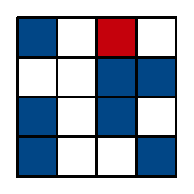
\includegraphics[width=0.35\columnwidth]{fig/map_tay_16_8.eps}
%\end{minipage}
}

\subfloat[Light core distribution of using ``lin \& greedy''
method.]{
\label{fig:boo-map-16}
%\begin{minipage}[b]{0.31\textwidth}
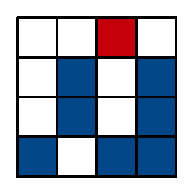
\includegraphics[width=0.35\columnwidth]{fig/map_boo_16_8.eps}
%\end{minipage}
}\qquad
% }
% \mbox{
\subfloat[Light core distribution of using ``random''
method.]{
\label{fig:ran-map-16}
%\begin{minipage}[b]{0.31\textwidth}
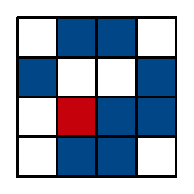
\includegraphics[width=0.35\columnwidth]{fig/map_ran_16_8.eps}
%\end{minipage}
}
\caption{Light core distribution estimation results of the 16-core system when light core number is $8$ and $f = 0.9$.}
\label{fig:map}
\end{figure}


We first test the accuracy of the proposed light cores distribution estimation method. Here we use the 16-core system as an example for demonstration and discussion. Results on systems with other core numbers are also collected and will be discussed later. To further demonstrate the effectiveness of the proposed light core distribution method, randomly generated light core distributions with light core number ranging from $1$ to $16$ are implemented (called "random" for short).

The estimated PPW results are shown in Fig. x to analyze the accuracy of different methods. To clearly show the results, we only plot the curves representing $f = 0.9$, $f$ is the fraction of the code that can be run in parallel. From Fig. x, we can see that the curve representing "lin-only" almost overlaps with that of the golden result. Besides, the curve representing "lin \& greedy" are close to the golden curve, showing small estimation error. While the curve representing "random" deviates greatly from the golden curve. Such observation means that implementing Taylor expansion based thermal models for PPW estimation is accurate, which can be verified by curve "lin-only". And further performing greedy based search strategy introduces small extra error as expected, but it can significantly reduce the estimation time as can be shown later. The PPW estimation error of "lin-only" is very small, which can be shown in Fig. x. While the PPW estimation error of "lin \& greedy" is larger, meaning the greedy based search strategy can boosting the estimation speed greatly by introducing reasonable error. The PPW estimation result of "random" deviates from that of the golden too much, which can be shown in Fig. x.

In addition to showing the PPW estimation results of different methods, we also plot the light core distribution maps of all methods when light core number is $8$ in Fig. x. The cores in blue and red are active during parallel computation process, while the cores in while are off. During sequential computation process, the core in red is active, and the cores in blue are in idle state. It is clear that the light core distributions of golden and "lin-only" are identical to each other. While the light core distribution of "lin \& greedy" differs from the golden one, and the reason is that the greedy based search strategy can only find the optimal solution based on the solution of previous step, which makes the solution sub-optimal. As the step number increases, the difference between the optimal solution and sub-optimal solution may increase. But as can be verified in our experiments, the PPW estimation of sub-optimal light core distribution only slightly degenerates than that of the optimal solution. 


\subsection{Speed and accuracy data of the proposed method}
We have graphically seen from Section $x$ that the new method has good accuracy. Now in this part, we show the speed and accuracy comparison results of the new method against the iterative method. Multi-core systems with core numbers from $9$ to $64$ are implemented.

Table $1$ records the speed and accuracy data of the proposed light core distribution estimation method comparing with iterative method. For estimation accuracy, the "lin-only" introduces small errors, because it is based on the linear approximation of static power at two Taylor expansion points. Errors given by "lin \& greedy" are slightly larger than those of the "lin-only" one, the reason is that greedy based search strategy can only find the sub-optimal solution.

Then let us look at the speed comparison in Table $1$. First, "lin-only" are several times faster than "ite" because it implements the linear thermal model to avoid the time-consuming iteration process. Then, "lin \& greedy" method can further greatly reduce estimation time. Due to the greedy based search strategy, we can magnificently speed up the estimation at the cost of a little accuracy. 

For multi-core systems with core number exceeding $16$, we cannot get the estimation results by implementing methods with brute force search strategy, for it consumes too much time and computation resource. In table $2$, we give the speed and PPW estimation data of the proposed light core distribution estimation method.

% Please add the following required packages to your document preamble:
% \usepackage{multirow}
\begin{table}[]
\centering
\caption{Accuracy and speed comparison of different light core distribution estimation methods.}
\label{my-label}
\begin{tabular}{ccccccc}
\hline
\multicolumn{1}{|c|}{\multirow{2}{*}{core \#}} & \multicolumn{1}{c|}{\multirow{2}{*}{method}}        & \multicolumn{1}{c|}{\multirow{2}{*}{f}} & \multicolumn{2}{c|}{\begin{tabular}[c]{@{}c@{}}PPW error\\ (\%)\end{tabular}}       & \multicolumn{1}{c|}{\multirow{2}{*}{\begin{tabular}[c]{@{}c@{}}time\\ (s)\end{tabular}}} & \multicolumn{1}{c|}{\multirow{2}{*}{\begin{tabular}[c]{@{}c@{}}speedup\\ vs ite\end{tabular}}} \\ \cline{4-5}
\multicolumn{1}{|c|}{}                         & \multicolumn{1}{c|}{}                               & \multicolumn{1}{c|}{}                   & \multicolumn{1}{c|}{max}                 & \multicolumn{1}{c|}{avg}                 & \multicolumn{1}{c|}{}                                                                    & \multicolumn{1}{c|}{}                                                                          \\ \hline
                                               &                                                     &                                         &                                          &                                          &                                                                                          &                                                                                                \\ \hline
\multicolumn{1}{|c|}{\multirow{9}{*}{9}}       & \multicolumn{1}{c|}{\multirow{3}{*}{ite}}           & \multicolumn{1}{c|}{1}                  & \multicolumn{1}{c|}{\multirow{3}{*}{NA}} & \multicolumn{1}{c|}{\multirow{3}{*}{NA}} & \multicolumn{1}{c|}{\multirow{3}{*}{1.24}}                                               & \multicolumn{1}{c|}{\multirow{3}{*}{NA}}                                                       \\ \cline{3-3}
\multicolumn{1}{|c|}{}                         & \multicolumn{1}{c|}{}                               & \multicolumn{1}{c|}{0.9}                & \multicolumn{1}{c|}{}                    & \multicolumn{1}{c|}{}                    & \multicolumn{1}{c|}{}                                                                    & \multicolumn{1}{c|}{}                                                                          \\ \cline{3-3}
\multicolumn{1}{|c|}{}                         & \multicolumn{1}{c|}{}                               & \multicolumn{1}{c|}{0}                  & \multicolumn{1}{c|}{}                    & \multicolumn{1}{c|}{}                    & \multicolumn{1}{c|}{}                                                                    & \multicolumn{1}{c|}{}                                                                          \\ \cline{2-7} 
\multicolumn{1}{|c|}{}                         & \multicolumn{1}{c|}{\multirow{3}{*}{lin-only}}      & \multicolumn{1}{c|}{1}                  & \multicolumn{1}{c|}{0}                   & \multicolumn{1}{c|}{0}                   & \multicolumn{1}{c|}{\multirow{3}{*}{0.35}}                                               & \multicolumn{1}{c|}{\multirow{3}{*}{3.54}}                                                     \\ \cline{3-5}
\multicolumn{1}{|c|}{}                         & \multicolumn{1}{c|}{}                               & \multicolumn{1}{c|}{0.9}                & \multicolumn{1}{c|}{0.01}                & \multicolumn{1}{c|}{0}                   & \multicolumn{1}{c|}{}                                                                    & \multicolumn{1}{c|}{}                                                                          \\ \cline{3-5}
\multicolumn{1}{|c|}{}                         & \multicolumn{1}{c|}{}                               & \multicolumn{1}{c|}{0}                  & \multicolumn{1}{c|}{0.20}                & \multicolumn{1}{c|}{0.05}                & \multicolumn{1}{c|}{}                                                                    & \multicolumn{1}{c|}{}                                                                          \\ \cline{2-7} 
\multicolumn{1}{|c|}{}                         & \multicolumn{1}{c|}{\multirow{3}{*}{lin \& greedy}} & \multicolumn{1}{c|}{1}                  & \multicolumn{1}{c|}{0.79}                & \multicolumn{1}{c|}{0.24}                & \multicolumn{1}{c|}{\multirow{3}{*}{0.10}}                                               & \multicolumn{1}{c|}{\multirow{3}{*}{12.4}}                                                     \\ \cline{3-5}
\multicolumn{1}{|c|}{}                         & \multicolumn{1}{c|}{}                               & \multicolumn{1}{c|}{0.9}                & \multicolumn{1}{c|}{0.71}                & \multicolumn{1}{c|}{0.22}                & \multicolumn{1}{c|}{}                                                                    & \multicolumn{1}{c|}{}                                                                          \\ \cline{3-5}
\multicolumn{1}{|c|}{}                         & \multicolumn{1}{c|}{}                               & \multicolumn{1}{c|}{0}                  & \multicolumn{1}{c|}{0.20}                & \multicolumn{1}{c|}{0.06}                & \multicolumn{1}{c|}{}                                                                    & \multicolumn{1}{c|}{}                                                                          \\ \hline
\multicolumn{1}{l}{}                           & \multicolumn{1}{l}{}                                & \multicolumn{1}{l}{}                    & \multicolumn{1}{l}{}                     & \multicolumn{1}{l}{}                     & \multicolumn{1}{l}{}                                                                     & \multicolumn{1}{l}{}                                                                           \\ \hline
\multicolumn{1}{|c|}{\multirow{9}{*}{16}}      & \multicolumn{1}{c|}{\multirow{3}{*}{ite}}           & \multicolumn{1}{c|}{1}                  & \multicolumn{1}{c|}{\multirow{3}{*}{NA}} & \multicolumn{1}{c|}{\multirow{3}{*}{NA}} & \multicolumn{1}{c|}{\multirow{3}{*}{596.32}}                                             & \multicolumn{1}{c|}{\multirow{3}{*}{NA}}                                                       \\ \cline{3-3}
\multicolumn{1}{|c|}{}                         & \multicolumn{1}{c|}{}                               & \multicolumn{1}{c|}{0.9}                & \multicolumn{1}{c|}{}                    & \multicolumn{1}{c|}{}                    & \multicolumn{1}{c|}{}                                                                    & \multicolumn{1}{c|}{}                                                                          \\ \cline{3-3}
\multicolumn{1}{|c|}{}                         & \multicolumn{1}{c|}{}                               & \multicolumn{1}{c|}{0}                  & \multicolumn{1}{c|}{}                    & \multicolumn{1}{c|}{}                    & \multicolumn{1}{c|}{}                                                                    & \multicolumn{1}{c|}{}                                                                          \\ \cline{2-7} 
\multicolumn{1}{|c|}{}                         & \multicolumn{1}{c|}{\multirow{3}{*}{lin-only}}      & \multicolumn{1}{c|}{1}                  & \multicolumn{1}{c|}{0}                   & \multicolumn{1}{c|}{0}                   & \multicolumn{1}{c|}{\multirow{3}{*}{124.38}}                                             & \multicolumn{1}{c|}{\multirow{3}{*}{4.79}}                                                     \\ \cline{3-5}
\multicolumn{1}{|c|}{}                         & \multicolumn{1}{c|}{}                               & \multicolumn{1}{c|}{0.9}                & \multicolumn{1}{c|}{0.13}                & \multicolumn{1}{c|}{0.08}                & \multicolumn{1}{c|}{}                                                                    & \multicolumn{1}{c|}{}                                                                          \\ \cline{3-5}
\multicolumn{1}{|c|}{}                         & \multicolumn{1}{c|}{}                               & \multicolumn{1}{c|}{0}                  & \multicolumn{1}{c|}{0.97}                & \multicolumn{1}{c|}{0.61}                & \multicolumn{1}{c|}{}                                                                    & \multicolumn{1}{c|}{}                                                                          \\ \cline{2-7} 
\multicolumn{1}{|c|}{}                         & \multicolumn{1}{c|}{\multirow{3}{*}{lin \& greedy}} & \multicolumn{1}{c|}{1}                  & \multicolumn{1}{c|}{3.83}                & \multicolumn{1}{c|}{1.62}                & \multicolumn{1}{c|}{\multirow{3}{*}{0.32}}                                               & \multicolumn{1}{c|}{\multirow{3}{*}{1863.50}}                                                  \\ \cline{3-5}
\multicolumn{1}{|c|}{}                         & \multicolumn{1}{c|}{}                               & \multicolumn{1}{c|}{0.9}                & \multicolumn{1}{c|}{3.52}                & \multicolumn{1}{c|}{1.51}                & \multicolumn{1}{c|}{}                                                                    & \multicolumn{1}{c|}{}                                                                          \\ \cline{3-5}
\multicolumn{1}{|c|}{}                         & \multicolumn{1}{c|}{}                               & \multicolumn{1}{c|}{0}                  & \multicolumn{1}{c|}{1.11}                & \multicolumn{1}{c|}{0.67}                & \multicolumn{1}{c|}{}                                                                    & \multicolumn{1}{c|}{}                                                                          \\ \hline
\end{tabular}
\end{table}





% Please add the following required packages to your document preamble:
% \usepackage{multirow}
\begin{table}[]
\centering
\caption{Speed and PPW estimation data of the proposed "lin \& greedy" method.}
\label{my-label}
\begin{tabular}{ccccc}
\hline
\multicolumn{1}{|c|}{\multirow{2}{*}{core \#}} & \multicolumn{1}{c|}{\multirow{2}{*}{f}} & \multicolumn{1}{c|}{\multirow{2}{*}{\begin{tabular}[c]{@{}c@{}}Optimal light\\ core number\end{tabular}}} & \multicolumn{1}{c|}{\multirow{2}{*}{\begin{tabular}[c]{@{}c@{}}Max\\ PPW\end{tabular}}} & \multicolumn{1}{c|}{\multirow{2}{*}{\begin{tabular}[c]{@{}c@{}}time\\ (s)\end{tabular}}} \\
\multicolumn{1}{|c|}{}                         & \multicolumn{1}{c|}{}                   & \multicolumn{1}{c|}{}                                                                                     & \multicolumn{1}{c|}{}                                                                   & \multicolumn{1}{c|}{}                                                                    \\ \hline
                                               &                                         &                                                                                                           &                                                                                         &                                                                                          \\ \hline
\multicolumn{1}{|c|}{\multirow{3}{*}{25}}      & \multicolumn{1}{c|}{1}                  & \multicolumn{1}{c|}{7}                                                                                    & \multicolumn{1}{c|}{0.0160}                                                             & \multicolumn{1}{c|}{\multirow{3}{*}{1.23}}                                               \\ \cline{2-4}
\multicolumn{1}{|c|}{}                         & \multicolumn{1}{c|}{0.9}                & \multicolumn{1}{c|}{2}                                                                                    & \multicolumn{1}{c|}{0.0157}                                                             & \multicolumn{1}{c|}{}                                                                    \\ \cline{2-4}
\multicolumn{1}{|c|}{}                         & \multicolumn{1}{c|}{0}                  & \multicolumn{1}{c|}{1}                                                                                    & \multicolumn{1}{c|}{0.0151}                                                             & \multicolumn{1}{c|}{}                                                                    \\ \hline
\multicolumn{1}{l}{}                           &                                         &                                                                                                           &                                                                                         & \multicolumn{1}{l}{}                                                                     \\ \hline
\multicolumn{1}{|c|}{\multirow{3}{*}{36}}      & \multicolumn{1}{c|}{1}                  & \multicolumn{1}{c|}{7}                                                                                    & \multicolumn{1}{c|}{0.0191}                                                             & \multicolumn{1}{c|}{\multirow{3}{*}{8.63}}                                               \\ \cline{2-4}
\multicolumn{1}{|c|}{}                         & \multicolumn{1}{c|}{0.9}                & \multicolumn{1}{c|}{4}                                                                                    & \multicolumn{1}{c|}{0.0184}                                                             & \multicolumn{1}{c|}{}                                                                    \\ \cline{2-4}
\multicolumn{1}{|c|}{}                         & \multicolumn{1}{c|}{0}                  & \multicolumn{1}{c|}{1}                                                                                    & \multicolumn{1}{c|}{0.0183}                                                             & \multicolumn{1}{c|}{}                                                                    \\ \hline
\multicolumn{1}{l}{}                           & \multicolumn{1}{l}{}                    & \multicolumn{1}{l}{}                                                                                      & \multicolumn{1}{l}{}                                                                    & \multicolumn{1}{l}{}                                                                     \\ \hline
\multicolumn{1}{|c|}{\multirow{3}{*}{49}}      & \multicolumn{1}{c|}{1}                  & \multicolumn{1}{c|}{12}                                                                                   & \multicolumn{1}{c|}{0.0223}                                                             & \multicolumn{1}{c|}{\multirow{3}{*}{30.25}}                                              \\ \cline{2-4}
\multicolumn{1}{|c|}{}                         & \multicolumn{1}{c|}{0.9}                & \multicolumn{1}{c|}{2}                                                                                    & \multicolumn{1}{c|}{0.0210}                                                             & \multicolumn{1}{c|}{}                                                                    \\ \cline{2-4}
\multicolumn{1}{|c|}{}                         & \multicolumn{1}{c|}{0}                  & \multicolumn{1}{c|}{1}                                                                                    & \multicolumn{1}{c|}{0.0207}                                                             & \multicolumn{1}{c|}{}                                                                    \\ \hline
\multicolumn{1}{l}{}                           & \multicolumn{1}{l}{}                    & \multicolumn{1}{l}{}                                                                                      & \multicolumn{1}{l}{}                                                                    & \multicolumn{1}{l}{}                                                                     \\ \hline
\multicolumn{1}{|c|}{\multirow{3}{*}{64}}      & \multicolumn{1}{c|}{1}                  & \multicolumn{1}{c|}{15}                                                                                   & \multicolumn{1}{c|}{0.0254}                                                             & \multicolumn{1}{c|}{\multirow{3}{*}{85.84}}                                              \\ \cline{2-4}
\multicolumn{1}{|c|}{}                         & \multicolumn{1}{c|}{0.9}                & \multicolumn{1}{c|}{1}                                                                                    & \multicolumn{1}{c|}{0.0237}                                                             & \multicolumn{1}{c|}{}                                                                    \\ \cline{2-4}
\multicolumn{1}{|c|}{}                         & \multicolumn{1}{c|}{0}                  & \multicolumn{1}{c|}{1}                                                                                    & \multicolumn{1}{c|}{0.0237}                                                             & \multicolumn{1}{c|}{}                                                                    \\ \hline
\end{tabular}
\end{table}

\subsection{Analysis}
We first analyze the properties of $Perf$ of a multi-core system in dark silicon. Here we use the 49-core system as an example for demonstration and discussion. In this case, the $Perf$ corresponds to the light core distributions in which the PPW is maximum. Noted, the Fred Pollack's performance efficiency rule is implemented, which states that, the performance of a processor that consumes $N$ times more transistors can only improve $\sqrt{T}$ times. We set the performance of a core in the 16-core system to be $1$.

\begin{figure}
\centering
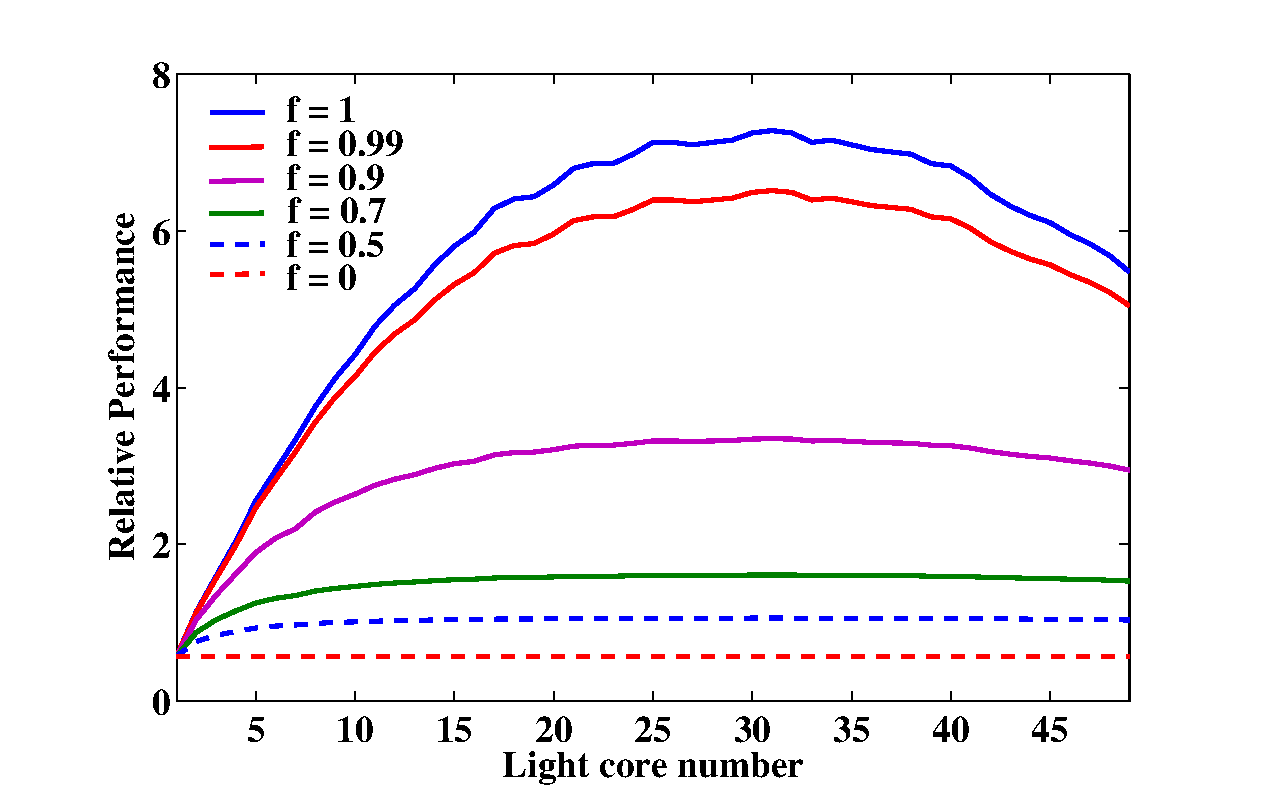
\includegraphics[width=1\linewidth]{fig/perf_boo_49.eps}
\caption{The relative performance of the 49-core system in dark silicon}
\end{figure}



\begin{figure}
\centering
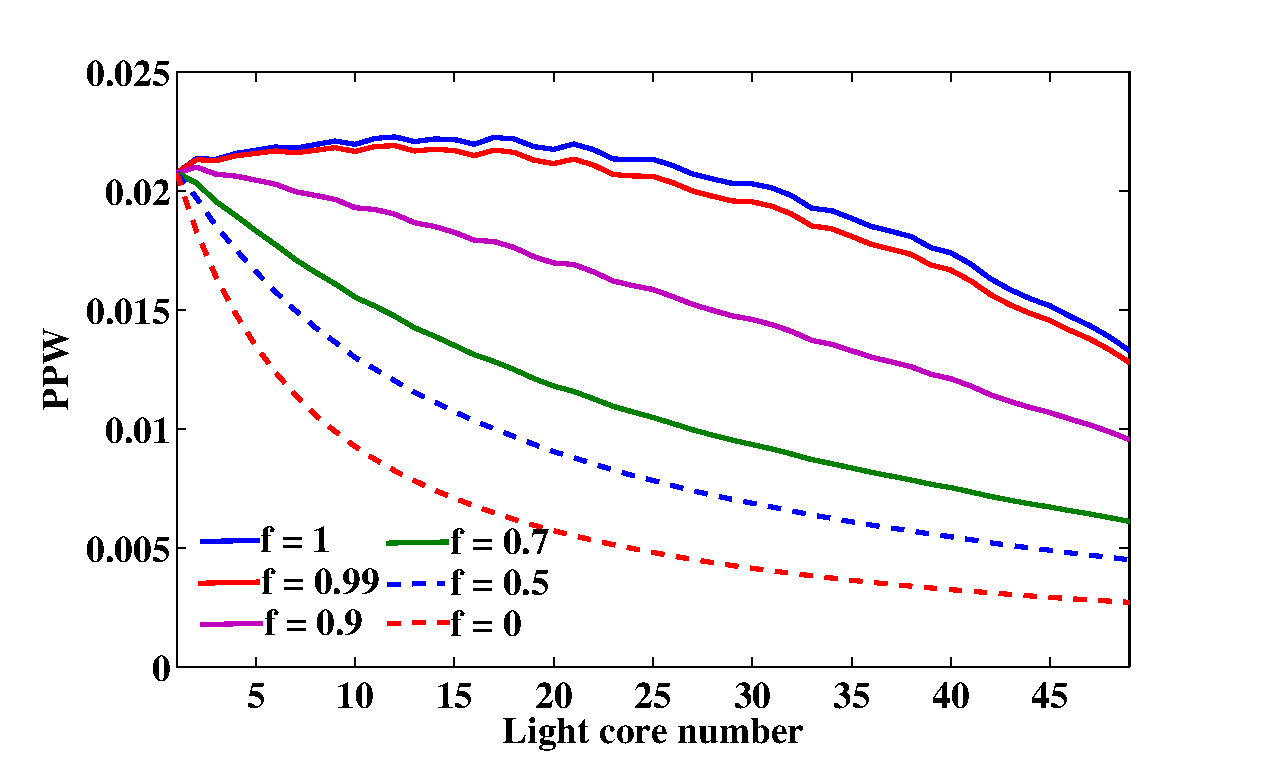
\includegraphics[width=1\linewidth]{fig/ppw_boo_49.eps}
\caption{The estimation of the PPW of the $49$-core system in dark silicon}
\end{figure}

As can be shown in Fig. x, the maximum $Perf$ of the 49-core system is $7.28$, where $f = 1$ and $n = 31$. However, as the number of light cores increase after the critical value of $31$, the $Perf$ would be worse, this is due to the performance deterioration resulting from DVFS. After certain light core number, the $Perf$ introduced by new light core would be less than the $Perf$ deterioration it causes to former light cores. Compared with the speedup promised by traditonal Amdahl's law with core number increasing, 

Next, we shall discuss the properties of PPW of a multi-core system in dark silicon. Here, we also use the 49-core system as an example for demonstration and discussion.

Fig. x shows the PPW of a 49-core system in dark silicon. We can see that for the cases where $f$ is relatively high, which means a large part of the code can be run in parallel, a optimal light core number $n$ which is higher than $1$ for maximum PPW exists. After this critical value of $n$, the PPW will decrease. The reason is that the relative performance of low fraction of parallel computation saturates much more easily, and increasing light core number after performance saturates will only drag down the energy efficiency.

It is also clear that the PPW of higher fraction of parallel computation decrease faster than that of lower fraction of parallel computation, the reason is that for sequential computation, increasing light core number only introduces an idle core, the performance degenerates only a little, while for parallel computation, the overall performance shall degenerate much more after certain light core number.

We can also see that higher $f$ means overall higher PPW, this is because higher fraction of parallel computation can provide more computing tasks to run on cores in parallel.
